%{{{ Preamble
\documentclass[usenatbib]{mnras}
\usepackage{graphicx}
\usepackage[export]{adjustbox}
\usepackage{bm}
\usepackage{amsmath}
\usepackage{amssymb}
\usepackage{algorithm}
\usepackage{algpseudocode}
\usepackage{subcaption}
\usepackage{layouts}
\usepackage{hyperref}
\usepackage[capitalise]{cleveref}
\usepackage{fancyvrb}
\usepackage{enumitem}
\usepackage{xcolor}
\usepackage{gensymb}
\usepackage[T1]{fontenc}
%}}}


\renewcommand\thesubsubsection{\Alph{subsubsection}.}
\newcommand{\nlive}{n_i}
\newcommand{\Like}{\mathcal{L}}
\newcommand{\DKL}{\mathcal{D}_\mathrm{KL}}
\newcommand{\logLmax}{\log \Like_\mathrm{max}}
\newcommand{\dG}{d_\mathrm{G}}


\title[\texttt{aeons}]{\texttt{aeons}: approximating the end of nested sampling}
\author[Z. Hu et al.]{Zixiao Hu\thanks{E-mail: zixiao.hu.09@gmail.com},$^{1,2}$  Artem Baryshnikov,$^{1,2}$  Will Handley\thanks{E-mail: wh260@cam.ac.uk}$^{1,2}$
\\
% List of institutions
$^{1}$Astrophysics Group, Cavendish Laboratory, J. J. Thomson Avenue, Cambridge, CB3 0HE, UK\\
$^{2}$Kavli Institute for Cosmology, Madingley Road, Cambridge, CB3 0HA, UK
}

\begin{document}
\label{firstpage}
\pagerange{\pageref{firstpage}--\pageref{lastpage}}
\maketitle


\begin{abstract}
    This paper presents analytic results on the anatomy of nested sampling, from which a technique is developed to estimate the run-time of the algorithm that works for any nested sampling implementation. We test these methods on both toy models and true cosmological nested sampling runs. The method gives an order-of-magnitude prediction of the end point at all times, forecasting the true endpoint within standard error around the halfway point.  
\end{abstract}

\begin{keywords}
methods: data analysis -- methods: statistical
\end{keywords}

\section{Introduction}
Nested sampling is a multi-purpose algorithm invented by John Skilling which simultaneously functions as a probabilistic sampler, integrator and optimiser \citep{skilling}. It was immediately adopted for cosmology, and is now used in a wide range of physical sciences including particle physics \citep{Trotta_2008}, materials science \citep{materials} and machine learning \citep{sparse_reconstruction}. The core algorithm is unique in its estimation of volumes by \textit{counting}, coupling together nested Monte Carlo integrals which makes high-dimensional integration feasible and robust. It also avoids problems that challenge traditional Bayesian samplers, such as posterior multi-modality and phase transitions.
\par
The order of magnitude run-time of an algorithm, that is, whether termination is hours or weeks and months away, is of high importance to the end user. Currently, existing implementations of nested sampling (e.g. \citealt{multinest, polychord, dnest, dynesty, ultranest, nessai,proxnest}) either do not give an indication of remaining run-time, or only provide crude measures of progress that do not directly correspond to the the true endpoint.
\par
This paper sets out a principled manner of endpoint estimation for nested sampling at each intermediate stage (as shown in \cref{fig:polychord_output}), the key idea being to use the existing samples to predict the likelihood in the region we have yet to sample from. We begin with an overview of nested sampling in \cref{sec:background}, followed by an examination of the anatomy of a nested sampling run to establish key concepts for endpoint prediction in \cref{sec:anatomy}. \cref{sec:endpoint} then outlines the methodology we use, including discussion and comparisons to previous attempts. Finally, \cref{sec:results} presents the results and discussions for toy and cosmological chains, before we conclude.
\begin{figure}
\begin{Verbatim}[frame=single, commandchars=\\\{\}]
\textcolor{red}{Predicted endpoint: 25054 +/- 242}
\textcolor{red}{Progress: [=================>########] 72%}
___________________
lives      |   500 |
phantoms   | 24310 |
posteriors | 18018 |
equals     |   245 |
-------------------
ncluster   =  1/1
ndead      =  18018
nposterior =  18018
nequals    =  249
nlike      =  4159049
<nlike>    =  491.04 (9.82 per slice)
log(Z)     =  -12.55 +/- 0.27
\end{Verbatim}
\caption{Output from \textsc{PolyChord} for a typical nested sampling run. The predicted endpoint, shown in red, is calculated using the method described in this paper.}
\label{fig:polychord_output}
\end{figure}

\section{Background}\label{sec:background}
We begin with a brief description of the nested sampling algorithm to establish the necessary notation. For a more comprehensive treatment, we recommend the original \citep{skilling} paper, the \citet{sivia} textbook, as well as the excellent technical review by \citet{Buchner_2023} and Nature review by \citet{physical_scientists}. 
\par
For a given likelihood $\mathcal{L}(\theta)$ and prior $\pi(\theta)$, nested sampling simultaneously calculates the Bayesian evidence
\begin{equation}\label{eq:evidence}
	\mathcal{Z} = \int \mathcal{L}\left(\theta\right)\pi(\theta)\ \mathrm{d}\theta
\end{equation}
while producing samples of the posterior distribution
\begin{equation}
	\mathcal{P}(\theta) = \frac{\mathcal{L}(\theta) \pi(\theta)}{\mathcal{Z}}.
\end{equation}
The algorithm operates by maintaining a set of $\nlive$ \textit{live points} sampled from the prior, which can vary in number throughout the run \citep{dynamic_ns}. At each iteration $i$, the point with the lowest likelihood is removed and added to a list of \textit{dead points} (illustrated in \cref{fig:dead_measure}). New points are then (optionally) drawn from the prior, subject to the constraint that they must have a higher likelihood than the current dead point~$\mathcal{L}_i$. Repeating the procedure leads to the live points compressing around peaks in the likelihood. If there are more births than deaths, the number of live points $n_i$ increases, whilst choosing to not generate new points reduces the number of live points. The exact creation schedule depends on the dynamic nested sampling strategy.
\par
The integral in \cref{eq:evidence} is then evaluated by transformation to a one-dimensional integral over the \textit{prior volume} $X$
\begin{equation}
	\mathcal{Z} = \int_0^1 \mathcal{L}(X)\ \mathrm{d}X \approx \sum_{i=1} \mathcal{L}_i\ \tfrac{1}{2}(X_{i-1}-X_{i+1}),
\end{equation}
where $X(\mathcal{L})$ is the fraction of the prior with a likelihood greater than $\mathcal{L}$. Whilst the likelihood contour $\mathcal{L}_i$ at each iteration is known, the prior volumes $X_i$ must be statistically estimated as follows: one can define a \textit{shrinkage factor} $t_i$ at each iteration $X_{i} = t_i X_{i-1}$, such that
\begin{equation}\label{eq:X_dist}
	X_i = \prod_{k=1}^i t_k.
\end{equation}
The $t_i$ are the maximum of $\nlive$ points drawn from $[0,1]$, so follow the distribution
\begin{equation}\label{eq:t_dist}
	P(t_i) = \nlive t_i^{\nlive-1},
\end{equation}
\begin{equation}\label{eq:t_moments}
    \langle\log t_i\rangle = -\frac{1}{\nlive}, \quad \mathrm{Var}(\log t_i) = \frac{1}{\nlive^2}.
\end{equation}
The algorithm terminates when an user-specified condition is met; a popular choice is when the evidence in the live points falls below some fraction $\epsilon$ of the accumulated evidence e.g. $10^{-3}$, which is proven to be a valid convergence criterion \citep{evans, Chopin_2010}.
Much of the existing literature treats this remaining evidence separately, for instance by estimating it as the termination $X$ multiplied by the average likelihood amongst the remaining live points. It is, however, quantitatively equivalent but qualitatively neater to consider termination as killing the remaining live points off one-by-one, incrementing the evidence exactly as during the run with decreasing $\nlive$ \citep{dynesty}.
\par
Uncertainties in the evidence are dominated by the spread in the prior volume distribution, and the simplest way to estimate them is by Monte Carlo sampling over sets of $\bm{t}$. As Skilling and others \citep{Chopin_2010, Keeton_2011} have shown, for any given problem the uncertainty in $\log \mathcal{Z}$ is proportional to $1/\sqrt{n_\mathrm{live}}$, so $n_\mathrm{live}$ sets the resolution of the algorithm.   

\section{The anatomy of a nested sampling run}\label{sec:anatomy}
The following sections act as an inventory of the information available to us at an intermediate iteration $i$, which we shall use to make endpoint predictions in \cref{sec:endpoint}. We present an anatomy of the progression of a nested sampling run in terms of the prior volume compression (\cref{sec:prior_volume}), the log-likelihood increase (\cref{sec:logL}), the inferred temperature (\cref{sec:temperature}), and the dimensionality of the samples (\cref{sec:dimensionality}).

\subsection{Prior volume}\label{sec:prior_volume}
The key feature of nested sampling is that the sampling is controlled by prior volume compression. The task is to find the posterior typically lying in a tiny fraction of the prior volume, a total compression which is quantified by the average information gain, or \textit{Kullback-Leibler divergence}:
\begin{equation}\label{eq:DKL}
   \DKL = \int \mathcal{P}(\theta) \log \frac{\mathcal{P}(\theta)}{\pi(\theta)}\ \mathrm{d}\theta. 
\end{equation}
The bulk of the posterior lies within a prior volume ${X = e^{-\DKL}}$, which is the target compression. From \cref{eq:t_moments} one gets there by iteratively taking steps of size ${\Delta \log X_i = -1/n_i}$, so that when we add up the contribution of each step in \cref{eq:t_moments} we get
\begin{equation}
    \langle\log X_i\rangle = -\sum_{k=1}^i \frac{1}{n_k}, \quad \mathrm{Var}(\log X_i) = \sum_{k=1}^i \frac{1}{n_k^2}.
\end{equation}
A steady step size in $\log X$ corresponds to a geometrically constant measure for the dead points, which is exactly needed to overcome the curse of dimensionality.
\begin{figure*}
\begin{center}
    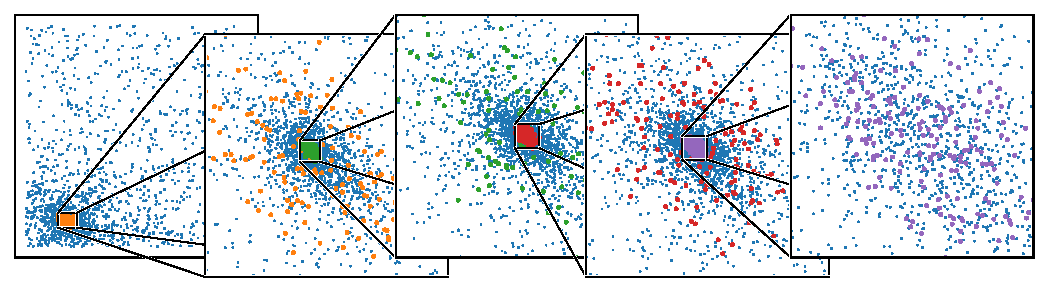
\includegraphics{figures/dead_measure_live.pdf}
\end{center}
\caption{The dead (small dots) and live points (larger dots) at several stages in a nested sampling run, recursively zoomed in. Note that the prior is taken to be uniform, which is reasonable because most nested sampling implementations require the prior to be provided as a transformation to the unit hypercube. The live points are uniform across the prior, while the dead points have a geometrically constant density.}
\label{fig:dead_measure}
\end{figure*}
\par
The same is not true for the live points, whose enclosed prior volume values are uniformly distributed, and by the comments in the penultimate paragraph of \cref{sec:background} have ${n_{i+k} = n_i-k}$. As a result, the maximum live point is found at 
\begin{equation}\label{eq:Xmin}
    \langle\log X_\mathrm{min}^{\mathrm{live}}\rangle = \langle\log X_i\rangle - \sum_{k=1}^{\nlive} \frac{1}{n_{i+k}} \approx -\frac{i}{\nlive} - \log \nlive - \gamma,
\end{equation}
with variance
\begin{equation}
    \mathrm{Var}(\log X_\mathrm{min}^{\mathrm{live}}) = \mathrm{Var}(\log X_i) + \sum_{k=1}^{\nlive} \frac{1}{n_{i+k}^2} \approx \frac{i}{\nlive^2} + \frac{\pi^2}{6}, 
\end{equation}
where the large $\nlive$ limit is taken for the approximation to the harmonic series, $\gamma$ being the Euler-Mascheroni constant.
\par
The live points therefore only get us a factor of $\log \nlive$ closer in volume to the posterior bulk. In other words, it is not until we are around $\log \nlive$ away from $\log X = -\DKL$ that the samples begin populating the posterior typical set. One can see from \cref{eq:DKL} that the divergence increases linearly with dimension, so for large dimensionalities and typical live point numbers $\lesssim 1000$, this does not happen until near the end of the run.
\par
The result is consistent with that in \citet{statmech}, which states that a spike at a volume smaller than $X_i/n_i$ will go undetected. Intuitively, it is because for a sharply peaked likelihood the live points are too diffuse to land there with any significant probability for most of the run. These results are summarised in \cref{fig:logX_distribution}
\begin{figure*}
\begin{center}
    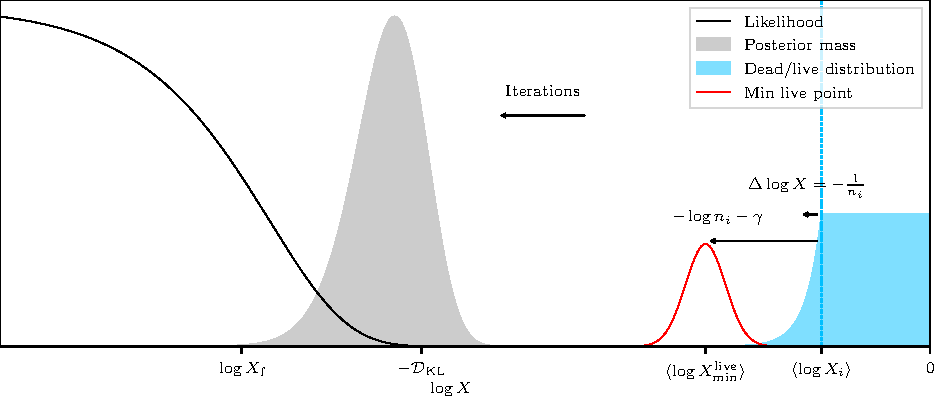
\includegraphics{figures/logX_distribution.pdf}
\end{center}
\caption{The distribution of the posterior mass in terms of $\log X$, the live points over the constrained prior and the smallest live point prior volume $\log X_\mathrm{min}^{\mathrm{live}}$ at an intermediate iteration $i$. For large values of $\DKL$ i.e. informative posteriors and/or large dimensionalities, the maximum live point is very far from the posterior bulk until the very end of the run. Note that the x-axis in this plot is $\log X$, so that the run proceeds from right to left to emphasise that the enclosed prior volume iteratively gets smaller. Plots of the sort from here onward will be in terms of $-\log X$, where the run will more naturally proceed from left to right. }
\label{fig:logX_distribution}
\end{figure*}

\subsection{Log-likelihood}\label{sec:logL}
We now consider the distribution of the samples in log-likelihood. To get an insight into the analytics, we will examine the case of the $d$-dimensional multivariate Gaussian likelihood with maximum point $\logLmax$ and length scale $\sigma$, situated in a uniform unit prior:
\begin{equation}\label{eq:logL_x}
    \log\Like = \logLmax - \frac{|\bm{x}|^{2}}{2\sigma^{2}}, \quad \bm{x} \in \mathbb{R}^{d}.
\end{equation}
This case is common and useful because many likelihoods are near-Gaussian, and most nested sampling implementations require the prior to be specified in terms of a transformation into the unit hypercube i.e. in prior probability units. Providing that $\sigma^d \ll 1$, the likelihood and posterior can be approximated as
\begin{equation}\label{eq:gaussian_logL}
    \log \Like = \logLmax - X^{2/d}/2\sigma^2,
\end{equation}
\begin{equation}
    \mathcal{P}(X) = \tfrac{1}{(2\pi\sigma^2)^{d/2}} e^{-X^{2/d}/2\sigma^2}, 
    \label{eqn:PX}
\end{equation}
which in terms of $\log\mathcal{L}$ becomes
\begin{equation}
    \mathcal{P}(\log\mathcal{L}) = \frac{1}{\Gamma\left(\frac{d}{2}\right)}e^{\log\mathcal{L}-\log\mathcal{L}_\mathrm{max}} (\log\mathcal{L}_\mathrm{max}-\log\mathcal{L})^{\frac{d}{2}-1}
\end{equation}
i.e. $2(\log\mathcal{L}_\mathrm{max}-\log\mathcal{L}) \sim \chi^2_{d}$, with mean and variance
\begin{equation}
    \langle\log\mathcal{L}\rangle_\mathcal{P} = \log\mathcal{L}_\mathrm{max} - \frac{d}{2},  \quad \mathrm{Var}(\log\mathcal{L})_\mathcal{P} = \frac{d}{2}.
\end{equation}
Given the prior volumes are uniform $X\sim U(0,1)$, the KL divergence in the $\sigma^d \ll 1$ limit is:
\begin{equation}
\mathcal{D}_\mathrm{KL} = -\frac{d}{2}\log 2 \Gamma(1+\tfrac{d}{2})^{2/d} \sigma^2.
\end{equation}

One can also derive the individual distributions for the live and dead points in log-likelihood. Note that this is merely the distribution of the $\log \Like$ \textit{values} of the points, without considering the associated prior volumes. The dead distribution is
\begin{equation}
    P(\log\Like) = \frac{\mathrm{d} \log X}{\mathrm{d} \log\Like} P(\log X) \propto \frac{d\:n_i}{2(\logLmax - \log\Like)},
\end{equation}
since the log-densities of the dead point prior volumes are proportional to the live point number at any given iteration. Meanwhile, the prior volumes enclosed by the live points (being independent samples) are always uniformly distributed, and so have the distribution 
\begin{multline}
	P(\log\mathcal{L}) = \frac{d}{2}\frac{(\log\mathcal{L}_\mathrm{max}-\log\mathcal{L})^{\frac{d}{2}-1}}{(\log\mathcal{L}_\mathrm{max}-\log\mathcal{L}_i)^{\frac{d}{2}}} \\
    [\log\mathcal{L}_i < \log\mathcal{L} <\log\mathcal{L}_\mathrm{max}].
    \label{eq:PL}
\end{multline}
\cref{fig:logL_distribution} shows the distinction between the distributions of the live and dead point values, as well as the posterior. 
\par
How much further do the live points penetrate in log-likelihood? We seek the distribution for the maximum likelihood of the live points, $\log\Like_{(n_i)}^{\mathrm{live}}$, where we have used the notation of order statistics to denote $x_{(k)}$ as the maximum of $k$ points.  For convenience, we will normalise the likelihoods as
\begin{equation}
    y = \frac{\log\mathcal{L}-\log\mathcal{L}_i}{\log\mathcal{L}_\mathrm{max}-\log\mathcal{L}_i}
    \label{eq:normalised_likelihood}
\end{equation}
so that $y=0$ corresponds to the most recent dead point at $\log\Like_i$ and $y=1$ to the maximum. The live point distribution simplifies to
\begin{equation}
    P(y) = \frac{d}{2}(1-y)^{\frac{d}{2}-1} \quad [0<y<1].
    \label{eq:Py}
\end{equation}
Using the result that the maximum of $n_i$ variables with cumulative distribution $F(y)$ follows $\frac{d}{dy}( 1- (1-F(y))^{n_i})$, we obtain
\begin{multline}
    P(y_{(n_i)}^\mathrm{live}) = \frac{n_i d}{2}(1-y_{(n_i)}^\mathrm{live})^{\frac{d}{2}-1}\left(1-(1-y_{(n_i)}^\mathrm{live})^{\frac{d}{2}}\right)^{n_i-1}\\ 
    [0<y_{(n_i)}^\mathrm{live}<1],
    \label{eq:Pyhat}
\end{multline}
which when analytically integrated to find its first and second moments give the mean and variance to be 
\begin{multline}
    y_{(n_i)}^\mathrm{live} \sim 1-\frac{\Gamma(1+\frac{2}{d})\Gamma(1+n_i)}{\Gamma(1+\frac{2}{d}+n_i)} \\
     \pm \left( \frac{\Gamma(1+n_i)\Gamma(1+\frac{4}{d})}{\Gamma(1+\frac{4}{d}+n_i)} - \frac{\Gamma(1+\frac{2}{d})^2 \Gamma(1+n_i)^2}{\Gamma(1+\frac{2}{d}+n_i)^2}\right)^{\frac{1}{2}}.
    \label{eq:ymax}
\end{multline}
In the large $d$, $n_i$ limit, taking the first and second order terms in the Taylor expansion simplifies the above expressions to 
\begin{align}
    \lim_{d\to\infty} y_{(n_i)}^\mathrm{live} &\sim \frac{2H_{n_i}}{d} \pm \left(\frac{2(\pi^2 - 6\Psi^{(1)}(1+n_i))}{3d^2}\right)^{\frac{1}{2}},
    \label{eq:ymaxd}\\
    \lim_{d,n_i\to\infty} y_{(n_i)}^\mathrm{live} &\sim \frac{2\log n_i}{d} \pm \sqrt{\frac{2}{3}}\frac{\pi}{d},
    \label{eq:ymaxdn}
\end{align}
where $\psi^{(1)}$ is the trigamma function and $H_{n_i}$ is the $n_i$th harmonic number. The final term is a very small fraction in high dimensions, showing that for Gaussian and near-Gaussian cases the live points are far from the posterior bulk until the very end.
\par
Alternatively, the same result arrives intuitively from the fact that at each step, $y$ increases by  
\begin{equation}\label{eq:dy}
    \lim_{\nlive \to \infty}\Delta y \approx \frac{\mathrm{d} y}{\mathrm{d}\log X} \Delta \log X = \frac{2}{d \nlive}, 
\end{equation}
so that by again summing the harmonic series, we get
\begin{equation}
    y_{(\nlive)}^{\mathrm{live}} \approx \frac{2\log \nlive}{d}.
\end{equation}
\cref{eq:dy} also implies that the normalised distance between the highest and second highest live point is roughly 
\begin{equation}
    y_{(\nlive)}^{\mathrm{live}} - y_{(\nlive - 1)}^{\mathrm{live}} \approx \frac{2}{d}.
\end{equation}
Before reaching the posterior bulk, $\logLmax - \log\Like_i > d/2$, so we must have
\begin{equation}
    \log \Like^{\mathrm{live}}_{(\nlive)} - \log \Like^\mathrm{live}_{(\nlive - 1)} > 1.
\end{equation}
In other words, for a Gaussian the highest likelihood point is always at least an order of magnitude greater than the second highest. It is therefore typically the case that nearly all of the posterior mass is concentrated in a single point, the maximum live point, until the very end of the run when the prior volumes have shrunk enough to compensate.
\par
The above results assume an exact Gaussian likelihood, which as discussed provides a reasonable first estimate for many physical likelihoods that are near-Gaussian. Further work can be done to generalise the analytics to non-Gaussians, though as we see in \cref{sec:results} results obtained via Gaussian assumptions can give the right order of magnitude.
\subsubsection*{Aside: nested sampling as a maximiser}
Previous literature \citep{Akrami_2010, Feroz_2011} has explored the potential for nested sampling to be used as a global maximiser, given its ability to handle multi-modalities. In particular, the latter authors emphasised that posterior samplers such as nested sampling find the bulk of the \textit{mass}, not the maximum of the distribution, but that this can be remedied by tightening the termination criterion. We now use the machinery we have developed to put this statement on a more quantitative footing, again examining the Gaussian case. 
\par
Let us take the current iteration to be the termination point with likelihood $\log\Like_\mathrm{f}$ and prior volume $X_\mathrm{f}$, so that
\begin{equation}
	\epsilon = \frac{\int_0^{X_\mathrm{f}} \mathcal{L}\ \mathrm{d}X}{\int_0^\infty \mathcal{L}\ \mathrm{d}X}.
\end{equation}
Note that we have assumed that prior effects are negligible (so $1\approx \infty$), and that $\epsilon \ll 1$ so that the denominator is approximately the accumulated evidence. Using \cref{eq:gaussian_logL}, we find the Gaussian termination condition in terms of lower incomplete gamma functions to be
\begin{equation}
\epsilon = 1- \frac{\Gamma_{d/2}\left(X_\mathrm{f}^{2/d}/2\sigma^2\right)}{\Gamma(d/2)}.
\end{equation}
Taking the $X_\mathrm{f}\ll (\sqrt{2}\sigma)^d$ limit (almost certainly valid at termination) we find
\begin{equation}\label{eq:Xf_approx}
    \lim_{X_\mathrm{f}\ll (\sqrt{2}\sigma)^d} \epsilon \approx \frac{X_\mathrm{f}}{(\sqrt{2}\sigma)^d \ \Gamma\left(1+\frac{d}{2}\right)} = \frac{(\log\mathcal{L}_\mathrm{max}-\log\mathcal{L}_\mathrm{f})^{\frac{d}{2}}}{\Gamma\left(1+\frac{d}{2}\right)}.
\end{equation}
We thus have an expression relating $\mathcal{L}_\mathrm{f}$ at termination to the termination fraction $\epsilon$. This becomes yet more pleasing in the large $d$ limit, since $\epsilon^{2/d}\to 1$, we find via a Stirling approximation:
\begin{equation}
    \lim_{d\to\infty} \log\mathcal{L}_\mathrm{f} \approx \log\mathcal{L}_\mathrm{max} - \frac{d}{2e}.
\end{equation}
In the event that we retain $\epsilon$, we replace $\frac{d}{2e}\to \frac{d}{2e}\epsilon^{2/d}$, allowing one to battle the $\frac{d}{2e}$ term exponentially as dimensions increase.
\par
Putting this together, taking $\mathcal{L}_i$ in \cref{eq:normalised_likelihood} to be $\mathcal{L}_\mathrm{f}$ and combining this with \cref{eq:ymaxdn}, we find
\begin{equation}
    \boxed{
        \log{\mathcal{L}}_\mathrm{max}^\mathrm{live} \approx \log\mathcal{L}_\mathrm{max} - \frac{d}{2e} + \frac{\log n_i}{e} \pm \frac{\pi}{\sqrt{6}e}
    },
\end{equation}
showing that Gaussian nested sampling chains will finish at a contour $d/2e$ away from the maximum log-likelihood. The final set of $n_i$ live points gets you $\log n_i/e$ closer, with a chance of getting $\sim\pi/\sqrt{6}e=0.472$ closer still at the $1\sigma$ interval. 
\par
Making the traditional termination criterion stricter therefore has limited returns in high dimensions, if it is ultimately still based on the remaining evidence. However, nested sampling still shrinks around the maximum exponentially, so provided a good alternative termination criterion is chosen, it will get there in reasonable time. 
\par
To quantify this statement, consider the number of iterations $\Delta i$ required to get from the posterior mean to the true maximum, which we will now calculate. At the posterior, we have roughly speaking
\begin{equation}
    (\log X, \log\Like) = (-\DKL, \logLmax - d/2).
\end{equation}
The prior volume $\log X_\delta$ at which the likelihood is within $\delta$ of the maximum of the Gaussian can then be found by inverting \cref{eq:gaussian_logL}:
\begin{equation}
    \log X_\delta = -\DKL - \frac{d}{2} \left(\log \frac{d}{2} - \log \delta\right),
\end{equation}
which corresponds to an additional
\begin{equation}\label{eq:delta_i_pd}
    \Delta i = \frac{nd}{2} \left(\log \frac{d}{2} - \log \delta\right)
\end{equation}
iterations after the bulk is reached, where $n$ is the harmonic mean of the number of live points. One would therefore expect a general distribution to take a similar order of magnitude of steps, that is $\mathcal{O}(\tfrac{n d }{2}\log \tfrac{d}{2})$ iterations to get from the usual nested sampling stopping point to within an $e$-fold of the maximum. A rule-of-thumb termination criterion could therefore be to run for at least $\tfrac{nd}{2}\log\tfrac{d}{2}$ iterations after the posterior is reached.
\par
We can also put compare this endpoint with the termination condition based on $\epsilon$. From \cref{eq:Xf_approx}, for any $d$, $n$ we have
\begin{equation}
    \log X_\mathrm{f} \approx \frac{d}{2}\log 2\sigma^2 + \log\epsilon + \log\Gamma\left(1+\frac{d}{2}\right),
\end{equation}
and using \cref{eq:gaussian_logL} to invert $\log\Like = \logLmax-\delta$ gives
\begin{equation}
    \log X_\delta=\frac{d}{2}\log 2\sigma^2+\frac{d}{2}\log\delta.
\end{equation}
Putting these together means that the difference in $\log X$ between the termination criterion based on evidence fraction $\epsilon$, and a point $\delta$ away from the maximum log-likelihood is
\begin{equation}
    \log X_\delta - \log X_\mathrm{f} \approx \frac{d}{2}\log\delta - \log\epsilon - \log\Gamma\left(1+\frac{d}{2}\right).
\end{equation}
Getting to within $\mathcal{O}(1)$ of the maximum after the termination criterion therefore takes an additional
 \begin{equation}
     \Delta i \approx n \left(\log\Gamma\left(1+\frac{d}{2}\right) - \log\frac{1}{\epsilon}\right)
\end{equation}
iterations. A larger dimension pushes the maximum away from the termination point, while a smaller $\epsilon$ brings it closer. Note the similarity of this equation to \cref{eq:delta_i_pd} via the Stirling approximation, and setting $\epsilon = 1/2$, approximately true at the posterior mean. 
\par
It automatically follows that the $\epsilon$ one should set to end the run $\mathcal{O}(1)$ away from the maximum is simply
\begin{equation}
    \boxed{\epsilon \approx \frac{1}{\Gamma\left(1 + d/2\right)}}.
\end{equation}
A summary of the distances between the notable points at the end of a run is shown in \cref{fig:logL_distribution}.

\begin{figure*}
\begin{center}
    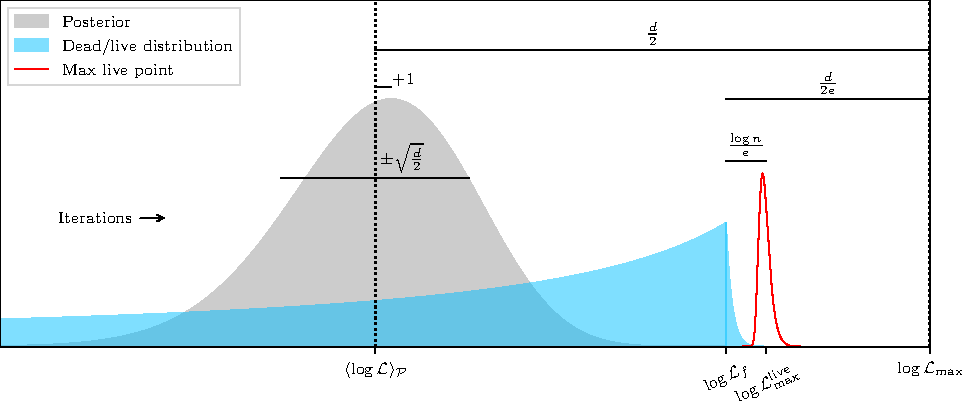
\includegraphics{figures/logL_distribution.pdf}
\end{center}
\caption{Distribution of samples as a function of $\log\mathcal{L}$, showing the posterior $\mathcal{P}(\log\mathcal{L})$, the distribution of the live points $\mathcal{\pi}(\log\mathcal{L} \mid \mathcal{L}>\mathcal{L}_i)$, and the distribution of the maximum likelihood live point $P(\log\mathcal{L}_\mathrm{max}^\mathrm{live})$. The distances are shown between these locations at the end of the run, the key takeaway being that in high dimensions the highest log-likelihood point of a nested sampling run is nowhere near the maximum in high dimensions.}
\label{fig:logL_distribution}
\end{figure*}


\subsection{Temperature}\label{sec:temperature}
\subsubsection*{Motivations}
In addition to $\log \Like_i$ and $\log X_i$, another useful piece of information at each iteration is the current \textit{temperature}, which we will now define.
\par
Bayesian inference is closely related to thermodynamics, for if one equates the parameters to microstates $i$, the negative log-likelihood to the microstate energy $E_i$, and the prior to the density of states $g_i$, then the posterior as given by the generalised Bayes' rule is the canonical ensemble at inverse temperature $\beta = 1/T$:
\begin{equation}
    p(E_i) = \frac{g_i e^{-\beta E_i}}{Z(\beta)} \quad \leftrightarrow \quad \mathcal{P}_\beta(\theta) = \frac{\Like^{\beta}(\theta)\pi(\theta)}{\mathcal{Z}(\beta)}.
\end{equation}
Nested sampling therefore calculates the partition function $Z(\beta)$, with the feature that it is agnostic to the temperature; because a nested sampling chain is invariant under monotonic transformations of the likelihood, one can get the posterior at any temperature by setting $\Like \to \Like^\beta$ without losing information.
\par
Transforming the likelihood with $\beta$ changes the termination point of the run, because the posterior mass is redistributed. In the middle of a run, there is therefore a temperature one can set which makes the current iteration the termination point. This `current temperature of termination' provides a measure of progress, marching from $0 \to 1$ as the run converges, though it is uncalibrated in the sense that knowledge of the current temperature gives no indication of when the final temperature $\beta = 1$ will be reached. It is of course dependent on the threshold $\epsilon$ chosen for the termination point, and we will label this $\beta$ as $\beta_\epsilon$ to distinguish it from other definitions of the temperature we will later discuss.
\par
Changing the termination point is perhaps the most obvious consequence of changing $\beta$, but transforming the posterior mass can be useful in other ways. $\beta$ is ultimately just an additional degree of freedom in a nested sampling run, to be set at any value one sees fit. The primary purpose for introducing it in this paper is that by redistributing the posterior mass like so, one can regularize the Bayesian model dimensionality of an intermediate set of samples, which provides crucial information about the likelihood and hence the termination point. This will be elaborated on in \cref{sec:dimensionality}; for now, we discuss several other `temperatures' relevant to nested sampling, including those introduced in previous literature.

\subsubsection{Microcanonical temperature}
As noted by \citet{demons}, thermal algorithms such as thermodynamic integration \citep{path_sampling} get the evidence by evolving through a series of canonical ensembles via some temperature schedule, or annealing schedule. Nested sampling instead maintains \textit{microcanonical} ensembles, which are the iso-likelihood contours. Instead of using temperature \citep{simulated_annealing, parallel_tempering} or energy \citep{wang_landau} as a control parameter, nested sampling chooses a series of ensembles with constant relative volume entropy $\Delta \log X$, which allows the algorithm to handle phase transitions \citep{baldock}.
\par
An obvious candidate for the current temperature is therefore the microcanonical temperature $\beta_\mathrm{M} = \partial S/\partial E$, where the volume entropy is $\log X$ and the energy is as usual $-\log \Like$. This gives the density of states; as discussed in Skilling's original paper,
\begin{equation}
    \beta_\mathrm{M}  = - \frac{\mathrm{d} \log X}{\mathrm{d} \log \Like} \Bigg\vert_{\log \Like_i}
\end{equation}
is the $\beta$ at which $\Like^{\beta} X$ peaks at $\log X_i$, if differentiability is assumed. If the posterior is symmetric as a function of $\log X_i$ about its peak, then this corresponds to $\beta_\epsilon = 1/2$.
\par
Its value can be easily obtained via finite difference of the $\log \Like$ and $\log X$ intervals, albeit subject to an arbitrary window size for the differencing. Indeed, material science applications \citep{Baldock_2017} use this estimator to monitor the `cooling' progress of nested sampling, with a window size of 1000 iterations.

\subsubsection{Canonical temperature}\label{sec:canonical_temperature}
Another temperature, considered by \citet{demons}, is the $\beta$ at which the energy of the current dead point (i.e. $-\log \Like_i$) is equal to the average energy of all the points, live and dead. One can obtain it by inverting 
\begin{equation}
    \langle \log \Like \rangle_{\mathcal{P}_\beta} = \log \Like_i
\end{equation}
to find the `canonical' temperature $\beta_\mathrm{C}$ for which the above equation is true. While $\beta_\mathrm{M}$ is derived from (the gradient of) a single contour, this temperature uses the entire ensemble. It has the desirable property that it rises monotonically with compression, in analogy to a monotonic annealing schedule.

\subsubsection{Bayesian temperature}\label{sec:bayesian_temperature}
We furthermore propose a temperature $\beta_\mathrm{B}$ that is obtained via Bayesian inference, which returns a distribution rather than a point estimate. Since each value of $\beta$ leads to a different likelihood $\Like^{\beta}$, one can consider the posterior distribution as a function of $\log X$ to be \textit{conditioned} on $\beta$. We can therefore write
\begin{equation}
   \mathcal{P}(\log X \mid \beta) = \frac{\Like^{\beta}(X) X}{\mathcal{Z(\beta)}}.
\end{equation}
What we would really like is the distribution of $\beta$ at the present iteration, so the natural step is to invert this via Bayes' rule;
\begin{equation}
    P\left(\beta \mid \log X_i\right) = \frac{\mathcal{P}\left(\log X_i \mid \beta\right) P\left(\beta\right)}{P\left(\log X\right)}.
\end{equation}
As with all Bayesian analyses, the distribution of $\beta$ is fixed up to a prior, which we choose to be uniform in $\beta$. The obtained temperatures are consistent with the previous two choices, which may seem oddly coincidental. In fact, closer inspection reveals that large values of $P(\beta \mid \log X_i)$ are the temperatures with the largest values of the posterior at the present $\log X_i$, normalised by the corresponding evidence. Thus the Bayesian temperature uses the same idea as the microcanonical one (which maximises the posterior), except here the spread in result is accounted for.

\subsubsection*{Comparisons}
\cref{fig:beta_posteriors} shows the posterior distribution as a function of $\log X$ for a 32-d spherical Gaussian when set to the above four temperatures, as known at a given iteration roughly 30\% through a run. Lower prior volumes are to the right, and 25 samples are taken from the prior volume distribution to capture the nested sampling uncertainties. When $\beta = 1$, the untransformed posterior is concentrated at the single point with the highest likelihood. This is no longer the case when $\beta$ is set to any of the other values, causing the posterior to have non-vanishing variance. The termination temperature can be seen to transform the posterior to have exactly $\epsilon$ of the total evidence to the right hand side of the current iteration (dotted black line). $\beta_\mathrm{M}$ makes the peak of the posterior with respect to $\log X$ coincide with the current iteration, and $\beta_\mathrm{C}$ produces a very similar result from its own criteria. 25 samples are taken from the distribution of the Bayesian temperature and the resultant posterior plotted for each, displaying a much broader range of uncertainty compared to the other plots.
\par
\cref{fig:beta_plots} then shows how these four temperatures evolve during the run (i.e. as a function of $\log X$) for two cases: one containing a classic slab-spike phase transition and one without. The behaviour of the former case is especially useful, because it is well-known to trouble temperature-based samplers. 
\par
In the case of a single phase all temperatures are consistent, with the exception that this only holds for $\epsilon \approx 0.5$ for the termination temperature. This is expected, since we can see from \cref{fig:beta_posteriors} that this choice of epsilon places the current iteration roughly at the peak of the posterior just as $\beta_M$ does. Other choices of $\epsilon$ shift the profile up and down. This user-dependence can offer more flexibility, but also be a disadvantage as an extra parameter to be tuned. The temperatures diverge, however, during a phase transition. Notably, with the exception of the canonical temperature they all \textit{decrease} then increase again, in contrast to a typically monotonic annealing schedule. It is also evident from the plots that $\beta_\mathrm{B}$ is the only temperature that incorporates a measure of uncertainty.
\begin{figure*}
\begin{center}
    \includegraphics{figures/beta_posteriors.pdf}
\end{center}
\caption{The posterior distribution at an intermediate point 30\% of the way through a nested sampling run for a 32$d$ spherical Gaussian, with the likelihood transformed from  $\Like \to \Like^{\beta}$ for several different choices of $\beta$. The untransformed posterior has all its weight at a single point. The other $\beta$ produce relatively similar transformations with finite posterior variance. Notably, the termination temperature is dependent on a manual choice of $\epsilon$, and the Bayesian temperature includes uncertainty in $\beta$ itself.}
\label{fig:beta_posteriors}
\end{figure*}

\begin{figure}
\begin{center}
    \includegraphics{figures/beta_plots.pdf}
\end{center}
\caption{Inferred temperatures using the termination ($\epsilon = 10^{-3}$), microcanonical, canonical and Bayesian definitions. The shaded region shows the $1-2\sigma$ uncertainties for the Bayesian temperature. $\beta_\epsilon$ is offset from the others, but can be shifted up and down depending on the chosen $\epsilon$. The other $\beta$ are all are consistent in a single phase, but differ during a phase transition.}
\label{fig:beta_plots}
\end{figure}
Despite the above theoretical justifications, one should remember the original motivation for introducing $\beta$ was to utilise the extra degree of freedom it provides, to transform the likelihood without losing information. As we will see in \cref{sec:choosing_the_best_temperature}, one can choose the exact definition depending on what is useful for the problem at hand.

\subsection{Dimensionality}\label{sec:dimensionality}
We can now use the inferred temperature to track how the effective dimensionality of the posterior changes throughout the run, which was previously inaccessible. \citet{Handley_2019} demonstrated that at the end of a run, a measure of the number of constrained parameters is given by the Bayesian model dimensionality $\dG$, defined as the posterior variance of the information content:
\begin{equation}\label{eq:d_G}
    \frac{\dG}{2} = \int \mathcal{P}(\theta) \left(\log \frac{\mathcal{P}(\theta)}{\pi(\theta)} - \DKL\right)^2 \: \mathrm{d}\theta
    = \langle \mathcal{I}^2 \rangle_\mathcal{P} - \langle \mathcal{I} \rangle^2_\mathcal{P}.
\end{equation}
As is discussed in \citet{Handley_2019}, $\dG$ holds valuable information about the posterior, measuring the number of spatial degrees of freedom in the posterior in the manner of principal component analysis, but without introducing arbitrary cut-off eigenvalues. It is exact in the case of a multivariate Gaussian likelihood that is small in length scale relative to the prior, so for non-Gaussian likelihoods $\dG$ can be considered the equivalent dimension if it were actually a Gaussian. Furthermore, it can be written as the posterior variance of the log-likelihood:
\begin{equation}
    \frac{\dG}{2} = \mathrm{Var}(\log\Like)_\mathcal{P}.
\end{equation}
Unfortunately, calculating this quantity in the middle of a run tends to return zero. That naturally follows from the results of \cref{sec:logL}, which shows that an intermediate set of samples typically have all their weight concentrated at a single point, the maximum live point, and a single point has vanishing variance. This behaviour continues practically until the run is close to termination. Re-weighting the likelihood by re-setting the temperature, however, leads this to no longer be the case. As shown in \cref{fig:beta_posteriors}, the posterior variance (and hence dimensionality) is zero at $\beta = 1$ but nonzero for the various other temperatures presented. 
\par
We find that the $\dG$ calculated from these transformed posteriors are exactly the Bayesian model dimensionalities of the \textit{true} posterior. \cref{fig:d_G_gaussians} demonstrates this using the microcanonical and Bayesian temperatures, on several spherical Gaussians for which the true value of $\dG$ is known; except for the earliest iterations, the right value is found to within standard error for all the likelhoods. The Bayesian temperature has slightly larger error bounds, as a more cautious estimate, but otherwise the estimates are consistent. 
\par
This provides a crucial piece of information, allowing us to access the Gaussian dimensionality of the true posterior before the run is complete. Before we discuss how this is can be used to aid endpoint estimation, we consider how the prior can affect the value of $\dG$ mid-run.  
\begin{figure*}
\begin{center}
    \includegraphics{figures/d_G_gaussians.pdf}
\end{center}
\caption{Bayesian model dimensionalities estimated throughout a run for spherical Gaussians of varying dimensions, which were not previously accessible before the end of a run because the posterior samples have vanishing variance. Calculating the value from the transformed likelihood $\Like \to \Like^{\beta}$, however, recovers the dimensionality of the final posterior before it is reached, which is shown in the above plots. Shading represents the $1-2\sigma$ uncertainties on the estimates $\hat{d}_\mathrm{G}$ of the true posterior dimensionality. Only the microcanonical and Bayesian temperatures are shown for clarity of comparison.}
\label{fig:d_G_gaussians}
\end{figure*}


\subsubsection*{Aside: Prior effects}\label{sec:prior_effects}
We now highlight the manner in which the prior limits our knowledge of the dimensionality of the posterior during a nested sampling run, and thus our estimate of the endpoint. A simple, but illustrative example is an elongated two-dimensional Gaussian, with parameters $(\theta_1, \theta_2)$, $\bm{\mu} = (0, 0)$, $\Sigma = \mathrm{diag}(0.8, 2.5\times10^{-9})$, prior $\theta_1 \sim U(0, 2)$, $\theta_2\sim U(-10^{-3}, 10^{-3})$. After transformation to the unit hypercube prior, the covariance matrix becomes
\begin{equation}
    \Sigma = \mathrm{diag}(0.2, 0.01)
\end{equation}
Transformation to the hypercube makes it manifest that compared to the posterior, the prior is narrow in the $\theta_1$ direction, and broad in the $\theta_2$ direction. The width of the prior \textit{relative} to the posterior plays a crucial part in how the samples evolve over a nested sampling run, which we will now see.
\par
Initially, the live point cloud is spread across the whole prior (\cref{fig:d_G_elongated_2D}, panel A). When it is time to find a point with a higher log-likelihood, it is much more likely to be in the $\theta_1$ direction because it is less well-constrained than $\theta_2$. The samples only compress in the  $\theta_1$ direction, and thus in this phase the live and dead points lie in a single-dimensional subspace of the full two-dimensional posterior, with $\dG = 1$ (\cref{fig:d_G_elongated_2D}, panel B). Eventually, the live point cloud converges around $\theta_1$ sufficiently so that it is just as likely to find a higher $\log\Like$ in either parameter direction. Only at this point does the point cloud shrink in both directions, lying in the full two-dimensional space of the posterior, with $d_G = 2$ (\cref{fig:d_G_elongated_2D}, panel C). 
\par
The key point is that in panel B, the live point cloud is actually one-dimensional. When comapred to a truly one-dimensional posterior (\cref{fig:d_G_elongated_1D}), at point B the samples look the same in all aspects. The consequence is that at point B, we fundamentally cannot know if there are more parameters `waiting' to be constrained, or if we have already found all the relevant directions. There are no clever inference tricks to get around it, in the same way that we cannot infer a `spike' from a slab and spike posterior when all the samples have yet to find the `spike'. Knowing the total number of parameters of the prior and likelihood to get the `parameter dimensionality' also isn't helpful, because the posterior dimensionality could be significantly different due to parameter degeneracies or non-Gaussian likelihoods.
\par
Therefore, unless the prior happens to be chosen to perfectly constrain each principal component of the posterior to the same degree, the prior choice will cause the nested samples to initially only occupy a subspace of the true posterior with a lower dimensionality, only eventually evolving to occupy the full space.
\begin{figure*}
\begin{center}
    \subfloat[a][]{\includegraphics{figures/d_G_elongated_2D_simple.pdf}\label{fig:d_G_elongated_2D}}
    \subfloat[b][]{\includegraphics{figures/d_G_elongated_1D_simple.pdf}\label{fig:d_G_elongated_1D}}
\end{center}
\caption{(a) Dimensionality estimates for a 2$d$ Gaussian that is elongated in one of its dimensions, with $1-2\sigma$ uncertainties shaded. The locations of the live points in the prior are shown at three stages, indicated by the connecting lines. As can be seen from the live point distribution, the samples only compress in a single direction until much later in the run, and early on it appears as if the other direction is completely unconstrained. (b) The same figure repeated for a 1$d$ Gaussian that is actually unconstrained in the other direction. At early iterations panel A and B, the live point distribution is identical to the $2d$ case, showing that early on the full posterior dimensionality is unknown and cannot be inferred. The Bayesian temperature was used here to transform the likelihood, but the other temperatures give similar results.}
\label{fig:d_G_elongated}
\end{figure*}
\par
If the widths of the posterior in different directions (in the unit hypercube) are well-separated, like the above case, we see step change in the Bayesian model dimensionality. If the length scales are close together, however, the change is more gradual. This can be seen when comparing the inferred dimensionality of two $6d$ Gaussians with similar $\DKL$, one with 
\begin{equation}\label{eq:elongated_separated}
    \Sigma_\mathrm{separated} = \mathrm{diag}(10^{-3}, 10^{-3}, 10^{-3}, 10^{-6}, 10^{-6}, 10^{-6}),
\end{equation}
and the other with 
\begin{equation}\label{eq:elongated_close}
    \Sigma_\mathrm{close} = \mathrm{diag}(10^{-2}, 10^{-3}, 10^{-4}, 10^{-5}, 10^{-6}, 10^{-7}),
\end{equation}
shown in \cref{fig:d_G_elongated_comparison}. Given arbitrary prior choices in real nested sampling runs, the length scales of high-dimensional posteriors in the unit hypercube are not necessarily well-separated, so a typical chain will have a dimensionality profile similar to the right-hand side of \cref{fig:d_G_elongated_comparison}.
\begin{figure}
\begin{center}
    \includegraphics{figures/d_G_elongated_comparison.pdf}
\end{center}
\caption{Estimated posterior dimensionality throughout a run for two 6$d$ covariant Gaussians. The left hand side has a steep separation of length scales between half of the parameters and the other half, while the right hand side has parameters that gradually shrink in length scale. These characteristics are reflected in the respective step-like and gradual evolutions of the sample dimensionalities.}
\label{fig:d_G_elongated_comparison}
\end{figure}
\par
If we sensibly assume that the existence of more parameters to constrain leads to a longer runtime, the fact that we under-estimate the dimensionality also means that early on, any endpoint algorithm tends to under-estimate the endpoint. This is something we will have to live with.

\section{Endpoint prediction}\label{sec:endpoint}
As described in \citet{supernest} and further explored in the talk and upcoming paper \citet{kcl_talk, scaling_frontier}, the time complexity of nested sampling is
\begin{equation}
    T \propto \langle \tfrac{1}{\nlive} \rangle^{-1} \times \langle \mathcal{T}\{ \Like(\theta) \} \rangle \times \langle f_\mathrm{sampler} \rangle \times \DKL.
\end{equation}
The first term is the harmonic mean of the number of live points $\sim\mathcal{O}(n_i)$, which depends on the live point schedule chosen by the user. The second term is the average time per likelihood evaluation. The third is the average number of evaluations required to replace a dead point with a live point at higher likelihood, which is given by the implementation. The final term is the Kullback-Liebler divergence~\cref{eq:DKL}, the compression factor required to get from the prior to the posterior. This term is generally outside of user control, in most cases \textit{a priori} unknown, and of principal interest in this section.
\par
Our aim is therefore first to quantify the amount of compression required to reach the endpoint at approximately $\log X = -\DKL$, which provides an estimate of the how far the sampler still needs to penetrate into the posterior. Once the required compression $\log X_\mathrm{f}$ is known, multiplying by the harmonic mean of the number of live points through the run gives the iteration count. Converting the number of nested sampling iterations to a run-time requires knowledge of how the sampling efficiency changes throughout the run, which we will not attempt to do because the variation is highly implementation-specific. 
\par
On the final point: the iteration progress is roughly proportional to the runtime progress when the sampling efficiency does not vary in order of magnitude. When that is not the case, the estimate will still be useful if the variation is known \textit{a priori}. For example, ellipsoidal samplers such as \textsc{MultiNest} and the MLFriends algorithm in \textsc{UltraNest} reduce in efficiency near the posterior bulk, so an impatient user who does not wish to expend the extra exponential effort for the final few percent can confidently halt earlier if they know they are already near the termination point.

\subsection{The termination prior volume}\label{sec:termination}
Making the above discussion more precise, we wish to find the compression factor $\log X_ \mathrm{f}$ at which the termination criterion is met, which is larger in magnitude than $\DKL$ (\cref{fig:logX_distribution}). The difficulty is that at an intermediate iteration we only know the posterior up to the maximum log-likelihood live point, which until just before the end is far from the posterior bulk. 
\par
In order to get an idea of where the true posterior bulk sits, we need to predict what the posterior looks like past the highest live point. We do this by \textit{extrapolating} the known likelihood profile; that is, the trajectory of $\Like(X)$ traced out by the live and dead points. 
One would never use this predicted posterior to perform inference, since more accuracy can always be achieved by simply finishing the run. However, we will demonstrate it is sufficient for making a run-time prediction for $\log X_\mathrm{f}$. 
\par
Quantitatively, this proceeds as follows: fit a function $f(X, \phi)$  with some parameters $\phi$ to the known likelihood profile, which allows us to express the prior volume we need to compress to as
\begin{equation}
	\Delta \mathcal{Z} = \epsilon \mathcal{Z}_\mathrm{tot},
\end{equation}
or equivalently
\begin{equation}\label{endpoint}
	\int_0^{X_\mathrm{f}} f(X, \phi)\ \mathrm{d}X = \epsilon \left( \int_0^{X_i} f(X, \phi)\ \mathrm{d}X + \mathcal{Z}_\mathrm{dead} \right),
\end{equation}
where $X_i$ is the volume of the iteration we have currently compressed to, and $\mathcal{Z}_\mathrm{dead}$ is the evidence we have accumulated up to this point. $X_\mathrm{f}$ can then be identified by solving the above equation either analytically or numerically. 
\par
Once $X_\mathrm{f}$ is known, the corresponding iteration count depends on the live point schedule. For example, in the constant $\nlive$ case $\log X$ decreases by $1/n$ at each iteration, so the total number of iterations $N_\mathrm{f}$ would be
\begin{equation}\label{eq:Nf}
	N_\mathrm{f} = - n\log X_\mathrm{f}.
\end{equation}


\subsection{How to extrapolate?}\label{sec:how_to_extrapolate}
The critical ingredient here is the function $\phi$ used to fit the likelihood profile $\Like(X)$, which should be simple enough to make fitting possible mid-run, but ideally also flexible enough to avoid strong biases. 
Previous work, such as the fitting procedure in the original Nelder-Mead simplex algorithm to estimate the Hessian \citep{nelder_mead}, and the BAMBI nested sampling paper \citep{Graff_2012}, suggest fast Gaussian approximations can be a good candidate for (online) modelling of likelihoods. The following method uses a similar approach, but unlike the previous schemes do not fit directly in parameter space.
\par
A key observation is that the Bayesian model dimensionality is the equivalent dimension of the posterior if it were actually Gaussian. Fitting a Gaussian of this dimension to the likelihood profile therefore makes a reasonable approximation to the true distribution, without explicitly assuming the form of the likelihood function. 
\par
The parameterisation of the Gaussian that we fit is the same as that given in \cref{sec:logL}, which we shall repeat here for clarity;
\begin{equation}\label{gaussian}
    f(X; \phi) = \logLmax - X^{2/d}/2\sigma^2
\end{equation}
The extrapolation then proceeds thus:
\begin{enumerate}[leftmargin=*]
    \item Find the current dimensionality ${d}^{(i)}_G$ of the posterior
    \item Take the live point profile and perform a least squares fit to \cref{gaussian}, stipulating that $d = {d}^{(i)}_G$ to infer $\logLmax$ and $\sigma$ 
    \item Use the likelihood predicted by these parameters to solve \cref{endpoint} for $X_\mathrm{f}$
\end{enumerate}
The advantage of fitting a Gaussian is that the procedure can be sped up analytically. Firstly, the least squares regression is trivial because analytic estimators exist; the cost function 
\begin{equation}\label{chi squared}
	C^2(\logLmax, \sigma) = \sum_i \left| \log \Like_i - f(X_i; \logLmax, \sigma) \right| ^2
\end{equation}
is minimised with respect to $(\logLmax, \sigma)$ when
\begin{equation}\label{eq:sigma}
    \sigma^2 = \frac{N \sum_i X_i^{4/d} - \left(\sum_i X_i^{2/d}\right)^2}{2 \sum_i \log \Like_i \sum_i X_i^{2/d} - 2N \sum_i X_i^{2/d}\log \Like_i },
\end{equation}
and
\begin{equation}\label{eq:logLmax}
    \logLmax = \frac{1}{N} \sum_i \log \mathcal{L}_i + \frac{1}{2N\sigma^2} \sum_i X_i^{2/d}.
\end{equation}
Secondly, the termination prior volume can also be obtained analytically. Rewriting \cref{endpoint} in terms of the Gaussian parameters gives
\begin{equation}
	\epsilon = \frac{\int_0^{X_\mathrm{f}} \Like_\mathrm{max} \exp\left(-X^{2/d}/2\sigma^2\right)\ \mathrm{d}X}{\int_0^{X_i} \Like_\mathrm{max} \exp\left(-X^{2/d}/2\sigma^2\right)\ \mathrm{d}X + \mathcal{Z}_\mathrm{dead}}.
\end{equation}
The integrals have the analytic solution
\begin{equation}
	\int_0^{X_k} \Like_\mathrm{max} \exp\left(-X^{2/d}/2\sigma^2\right)\ \mathrm{d}X = \frac{d}{2} \cdot \left(\sqrt{2}\sigma\right)^d \cdot \gamma_k
\end{equation}
where $\gamma_k = \Gamma_{d/2}\left(X_k^{2/d}/2\sigma^2\right)$ is the lower incomplete gamma function. After taking the inverse of  $\gamma$ and a few more steps of algebra, we arrive at
\begin{equation}
    \log X_\mathrm{f} = \frac{d}{2}\log 2\sigma^2	+ \log \Gamma^{-1}_{d/2} \left(\epsilon \gamma_i+ \frac{\epsilon\mathcal{Z}_\mathrm{dead}}{ \left( 2\sigma^2 \right)^{d/2}\Like_\mathrm{max}}\right),\label{eq:xf}
\end{equation}
and $N_\mathrm{f}$ is then computed with \cref{eq:Nf}. Intuitively, the above procedure can be thought of as inferring the number of constrained parameters, then extrapolating them up to find the point at which they will be fully constrained. 
\par
Uncertainties in the final estimate are obtained by drawing many samples from the distribution of $\dG$ at the current iteration, and repeating step two for each. One might wonder why we do not obtain $d$ via least squares regression together with the other parameters; extensive testing has shown this approach to be far less stable.
\par
Thus far, we have not yet specified which temperature we should use to regularize $d_G^{(i)}$. We will now empirically assess the performance between the different temperatures across several test likelihoods.

\subsection{Choosing the best temperature}\label{sec:choosing_the_best_temperature}
We estimate the endpoint using the above procedure for three previously discussed test likelihoods, each in a unit hypercube prior:
\begin{enumerate}[leftmargin=*]
    \item Spherical Gaussian; $\sigma = 10^{-3}$
        \begin{equation}
        \log \Like = -\frac{|\bm{x}|^2}{2\sigma^2}, \quad \bm{x} \in \mathbb{R}^{32}
        \end{equation}
    \item Elongated Gaussian, two well-separated length scales 
        \begin{equation}
            \log\Like = -\frac{1}{2} \bm{x}^\intercal \Sigma^{-1}\bm{x}, \quad \bm{x} \in \mathbb{R}^6
        \end{equation}
        \begin{equation*}
            \Sigma_\mathrm{separated} = \mathrm{diag}(10^{-3}, 10^{-3}, 10^{-3}, 10^{-6}, 10^{-6}, 10^{-6}),
        \end{equation*}
    \item Elongated Gaussian, gradually changing length scales
        \begin{equation}
            \Sigma_\mathrm{close} = \mathrm{diag}(10^{-2}, 10^{-3}, 10^{-4}, 10^{-5}, 10^{-6}, 10^{-7}).
        \end{equation}
\end{enumerate}
Results are shown in \cref{fig:beta_endpoint_comparison}. Broadly speaking, the performance is similar, which is expected since the temperatures themselves are relatively consistent with each other (\cref{fig:beta_plots}).
\par
No estimates can be calculated for the termination temperature very early on in the run, because there is no choice of $\beta$ that will make the current iteration the termination point. For example, this is certainly true when $X_i > \epsilon$.
\par
We choose to use the Bayesian temperature in our implementation from this point onwards, because it incorporates the extra degree of uncertainty in the temperature itself, and this broader account of uncertainty is helpful when we are estimating endpoints using limited information. However, the choice is to some degree one of personal taste, and it remains reasonable to make estimates with the others.
\begin{figure*}
\subfloat{\includegraphics{figures/beta_endpoint_comparison_gauss_32.pdf}\label{gauss_32}}
\newline
\subfloat{\includegraphics{figures/beta_endpoint_comparison_correlated_6d.pdf}\label{elongated_gaussian_separated}}
\newline
\subfloat{\includegraphics{figures/beta_endpoint_comparison_correlated_6d_close.pdf}\label{elongated_gaussian_close}}
\caption{Endpoint estimates obtained from the procedure outlined in \cref{sec:how_to_extrapolate}, using different $\beta$ to regularize the $\dG$. The true endpoints are shown in dotted red, while the estimates with their $1-2\sigma$ uncertainties are shaded in blue. Progress is measured in terms of the compression $-\log X$ along the x-axis, while the estimates on the y-axis are in terms of the predicted final compression $-\log \hat{X}_\mathrm{f}$. The estimates are broadly consistent, but notable differences include the failure of the termination temperature to obtain estimates at early iterations, and the larger uncertainty bounds of the Bayesian temperature.}
\label{fig:beta_endpoint_comparison}
\end{figure*}



\subsection{Alternative approaches}
More comprehensive Bayesian approaches, perhaps including \textit{a priori} information about the likelihood or greater flexibility in the fitting function, could likely perform better than what we have just presented. However, such methods would not befit \textit{run-time} prediction which has a much more limited computational budget, hence the more pragmatic approach we have adopted. Here, we discuss as a benchmark alternative approaches to endpoint estimation that have a comparable computational complexity.
\subsubsection{Integral progress}
An alternative approach used in \textsc{Ultranest} \citep{ultranest} derives a progress bar based on the fraction of the accumulated integral compared to the remaining integral, approximated as 
\begin{equation}\label{eq:integral_progress}
    \mathcal{Z}_\mathrm{rem} \approx \Like_\mathrm{max}^{\mathrm{live}} X_i.
\end{equation}
This has a several shortcomings. First, run-time is proportional to compression rather than accumulation of the integral, since it takes just as long to traverse the width of the bulk as it does any other width. Second, because of the point-like nature of the posterior mid-run, the remaining integral approximated as such holds nearly all of the evidence, so the relative fraction of the accumulated and remaining evidence is almost zero for most of the run. Finally, approximation \cref{eq:integral_progress} is always an underestimate, because as previously found the maximum live point is generally nowhere near the true maximum. This approach can be useful in low dimensions when the live points are always near the maximum, but in general is less reliable.

\subsubsection{Extrapolating evidence increments}
Seasoned watchers of nested sampling runs might be curious how the method compares to simply extrapolating the increments of evidence to roughly estimate when the evidence converges. At an intermediate stage of the run, the most recent outputs look something like that shown in the first two columns of the table in \cref{fig:inc_extrapolate} (which in this case was a real run for a spherical Gaussian with $d = 16$, $\sigma = 0.01$). The right hand side of \cref{fig:inc_extrapolate} plots the gain in log-evidence at every 500 iterations, then extrapolates them with a linear and exponential profile. This is then used to calculate the point at which the gain is so small that the termination condition is met, shown separately for the linear and exponential extrapolations.
\par
Compared to the true endpoint (found by completing the run), the linear extrapolation is clearly an underestimate, since it fails to account for the long tail of the nonlinear profile. The increments are also not exactly exponential, since the exponential fit leads to a large over-prediction. The predicted endpoint over the course of a run, as shown in \cref{fig:inc_predictions}, shows the same result. One might expect an average to be more accurate, but this tends to be biased towards the exponential prediction, and there is no obvious choice of weighting that would fix this.
\par
More importantly, we find that for real likelihoods which have an element of noise the extrapolation often diverges, for instance when the increments do not monotonically decrease. Directly extrapolating the evidence increments is therefore far less stable than the previous method, and generally not a reliable method for prediction.
\begin{figure}
\begin{adjustbox}{valign=t, scale=0.7}
\subfloat{\begin{tabular}{|c|c|c|}
\hline
iteration & log Z  & $\Delta\log Z$   \\
\hline
5000 & -1435.8 & 190.8 \\
5500 & -1264.6 & 171.2 \\
6000 & -1123.7 & 140.9 \\
6500 & -991.5 & 132.2 \\
7000 & -885.0 & 106.6 \\
7500 & -790.3 & 94.7 \\
8000 & -702.6 & 87.7 \\
8500 & -619.7 & 82.9 \\
9000 & -551.8 & 67.9 \\
9500 & -492.7 & 59.1 \\
\hline
\end{tabular}}
\end{adjustbox}
\quad
\begin{adjustbox}{valign=t, scale=0.9}
    \subfloat{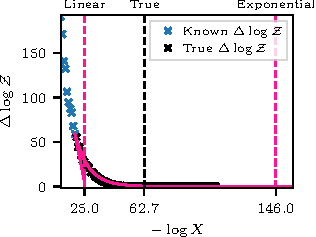
\includegraphics{figures/inc_extrapolate.pdf}}
\end{adjustbox}
\caption{Extrapolating the increases in evidence $\Delta \log \mathcal{Z}$ to predict the endpoint. The left column shows the most recent ten outputs from a nested sampling run currently at $n_\mathrm{dead} = 10,000$, together with the difference every 500 iterations, which appear to converge at a steady rate. The right hand side plots these past 10 increments (blue) as a function of the compression $-\log X_\mathrm{f}$, and attempts to extrapolate them via a linear and exponential profile (pink). This is used to predict when the increment will be small enough for the termination condition to be met (dashed pink). The true progress of the increments, obtained after completing the run, is plotted in black.}
\label{fig:inc_extrapolate}
\end{figure}
\begin{figure}
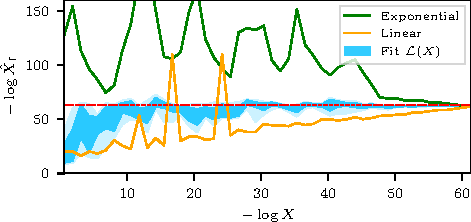
\includegraphics{figures/inc_predictions.pdf}
\caption{Endpoint predictions for a spherical Gaussian, with $1-2\sigma$ uncertainties shaded. Extrapolating the evidence increments in a linear/exponential manner under/over-predicts the endpoint, both of which perform considerably worse than the method of extrapolating the likelihood.}
\label{fig:inc_predictions}
\end{figure}

\section{Results}\label{sec:results}
We now test the approach established in the previous section on a range of distributions, beginning by considering a series of toy examples to explore the capabilities and limitations of the method, before presenting results for real cosmological chains.
\subsection{Toy examples}\label{sec:logXfs_toy}
Throughout the toy examples we make use the perfect nested sampling~\citep{Keeton_2011,2018BayAn..13..873H} framework implemented in \textsc{anesthetic}~\citep{anesthetic}.
\subsubsection{Spherical Gaussians}
Predictions for spherical Gaussians of various dimensions are shown in \cref{fig:logXfs_gaussian} as a benchmark for when fitting a Gaussian distribution is exact. In all endpoint prediction plots, the shading indicates the $1-2\sigma$ uncertainties. All were run with $\nlive = 500$ except for one $\nlive=2000$ for comparison, with each Gaussian having a width of $\sigma = 0.01$. The correct endpoint is recovered to within standard error at all points except the very beginning, when the parameters have hardly been constrained. 
\par
One can see from the $\log\Like-\log X$ plots in \cref{fig:logL_logX_plots} that the extrapolated likelihood is a good fit to the true likelihood, as expected from a spherical Gaussian. We also note that as with nested sampling in general, increasing $\nlive$ improves the resolution and reliability of the inferences, as indicated by the middle two plots of \cref{fig:logXfs_gaussian}.
\begin{figure*}
\begin{center}
    \includegraphics{figures/logXfs_gaussian.pdf}
\end{center}
\caption{Endpoint predictions for a spherical Gaussian run with $\nlive=500$ (except for the third plot from left). The true endpoints are shown in dotted red, while the estimates with their $1-2\sigma$ uncertainties are shaded in blue. Progress is measured in terms of the compression $-\log X$ along the x-axis, while the estimates on the y-axis are in terms of the predicted final compression $-\log \hat{X}_\mathrm{f}$. The correct endpoint is obtained for all but the earliest iterations, and the uncertainty is controlled by the number of live points, which can be seen from the two $d = 16$ plots.}
\label{fig:logXfs_gaussian}
\end{figure*}

\subsubsection{Correlated Gaussians}\label{sec:logXfs_correlated}
We also observe the effect of introducing different length scales and correlations to the Gaussian, generically 
\begin{equation}
    \log\Like = - \frac{1}{2} \bm{x}^{\intercal} \Sigma^{-1} \bm{x}, \quad \bm{x} \in \mathbb{R}^{d}.
\end{equation}
Again, all are run with a constant number of 500 live points. Starting from the left of \cref{fig:logXfs_correlated}, the first chain has the covariance matrix given in \cref{eq:elongated_separated}, featuring three parameters with $\sigma^2 = 10^{-3}$ and three with $\sigma^2=10^{-6}$. The endpoint predictions are step-like; as discussed in \cref{sec:prior_effects}, it only jumps to the correct endpoint when the prior is compressed enough to sample the $\sigma^2=10^{-3}$ parameters, which are initially better constrained by the prior. The second run from the left has the same $6d$ covariance matrix, except the three $\sigma^2=10^{-3}$ parameters are made completely unconstrained, so that the posterior only has three constrained parameters. The corresponding endpoint matches that obtained at early stages in the full $6d$ posterior, meaning that at those early stages the two cases are impossible to distinguish, and underprediction cannot be avoided.
\par
Equivalently, one can consider the inaccuracy as a breakdown of the approximation that takes the Gaussian likelihood \cref{eq:logL_x} to the fitting function \cref{eq:gaussian_logL}, which only holds when the prior is wide compared to the posterior. Since the live points resemble the prior in the beginning of the run, and some parameters are constrained before others, the approximation may only hold for some of the parameters, leading to the $\log\Like-\log X$ curve having a lower dimensionality at the start.
\par
The third chain from the left ($\Sigma$ given in \cref{eq:elongated_close}) then shows the effect of `smoothing' the parameter variances, so that they step down from $10^{-2}$ to $10^{-7}$ one power of ten at a time. Mirroring the behaviour shown in \cref{fig:d_G_elongated_comparison}, the predictions gradually converge to the truth as those parameters with narrower priors are discovered in gradual succession, instead of making a sudden jump. Finally, the fourth chain from the left rotates the covariance matrix in \cref{eq:elongated_separated} by $30\degree$, demonstrating that the above behaviour persists when the `principal components' of the posterior are no longer parallel to the parameter axes.
\par
All of these chains nevertheless surmise the correct endpoint by about halfway, and always give the right order of magnitude. The $\log\Like-\log X$ plot at 30\% of the way through for the elongated Gaussian (second from the left in \cref{fig:logL_logX_plots}) shows that the fitted profiles are of the same shape as the true likelihood, since both are Gaussian. However, the extrapolation undershoots because as discussed, prior effects initially cause the sample dimensionality to be lower than the true dimensionality of the posterior. 
\begin{figure*}
\begin{center}
    \includegraphics{figures/logXfs_correlated.pdf}
\end{center}
\caption{Endpoint predictions for four $6d$ Gaussians with different covariance matrices. From the left, the first chain has parameters with two distinct length scales, so the predictions show a step-like trend due to prior effects. The second chain has three unconstrained parameters in place of three parameters in the first chain, so the predictions are identical to the early stages of the first chain. The third plot shows that if the parameters have a gradual spectrum of length scales, the prior effects fade away more gradually, reflected in the gradual convergence of the estimates. The fourth and final plot shows that the prior effects, most evident in the chains with two distinct length scales, persist when the posterior components are not parallel to the parameter axes.}
\label{fig:logXfs_correlated}
\end{figure*}

\subsubsection{Non-Gaussian likelihoods}
We now look at how well the extrapolation procedure works when the likelihoods are significantly non-Gaussian, since one might expect fitting a Gaussian to fail. 
First, we consider the 10-dimensional Rosenbrock function with $a = 1$,  $b = 100$:
\begin{equation}
    \log \Like = - \sum_{i = 1}^{9} \left(a - x_i\right)^2 + b\left(x_{i+1} - x_i^2\right)^2, \quad \bm{x} \in \mathbb{R}^{10},
\end{equation}
which is important because it has strong correlations between the parameters which do not factorize, such that the concept of dimensionality is less clear. Another case that might be expected to cause problems is the pathological Cauchy distribution, which is far from a Gaussian:
\begin{equation}
    \log\Like = - \frac{1+d}{2} \log \left( 1 + \frac{|\bm{x}|^2}{\gamma^2}\right), \quad \bm{x} \in \mathbb{R}^8
\end{equation}
which we test with $\gamma = 10^{-4}$ and $d = 8$. Results are shown in \cref{fig:logXfs_non_gaussian}. The Rosenbrock initially underestimates the endpoint, getting the right answer with around 5,000 iterations of 15,529 remaining, though the prediction at worst hovers at around 60-70\% of the actual run time. Prior effects contribute to the under-estimation in the same manner as all of the previous non-spherical likelihoods, but \cref{fig:logL_logX_plots} reveals that the relatively poor fit (but still reasonable) of a Gaussian to the Rosenbrock function also plays a role.
\par
The Cauchy also under-predicts at first, obtaining the correct endpoint within standard error by about halfway through its 39,236 iterations. The posterior here is spherically symmetric, so compression is isotropic and the prior affects all parameters equally. Because there are no associated under-estimates of the posterior dimensionality, the inaccuracies are solely due to the poor fit of a Gaussian to a Cauchy, which can be seen in the rightmost plot of \cref{fig:logL_logX_plots} as much more drastic than the other likelihoods; the Bayesian model dimensionality is itself less stable for Cauchy likelihoods. Nevertheless, the right order of magnitude is obtained at all times, so this remains sufficient for most use-cases. The Cauchy is also a pathological case, and the same problem does not in practice appear for more realistic examples, as we shall see in the next section.
\begin{figure*}
\begin{center}
    \includegraphics{figures/logXfs_non_gaussian.pdf}
\end{center}
\caption{Endpoint predictions throughout for two non-Gaussian likelihoods, a Rosenbrock and a Cauchy, with the red dotted line showing the true endpoint and the blue shading indicating the $1-2\sigma$ uncertainties. The endpoint is initially underestimated for the Rosenbrock, due to a combination of prior effects and the breaking down of the Gaussian model. The Cauchy is also underestimated for the first half of the run, but this is solely a limitation of the Gaussian approximation because the likelihood is spherically symmetric.}
\label{fig:logXfs_non_gaussian}
\end{figure*}

\begin{figure*}
\includegraphics{figures/logL_logX_plots.pdf}
\caption{Fitted extrapolations compared to the true likelihood for four different test likelihoods. The live points at 30\% through the run for each example are fitted a to Gaussian, extrapolated to the higher likelihoods that have not yet explored, and compared to the ground truth. It is clear that truly Gaussian likelihoods are modelled well, while the model deteriorates with increasing non-Gaussianity (seen in the Rosenbrock and Cauchy likelihoods).}
\label{fig:logL_logX_plots}
\end{figure*}


\subsection{Cosmological examples}\label{sec:cosmological_examples}
Finally, we evaluate the method on real cosmological chains. \cref{fig:logXfs_lcdm} presents endpoint estimates (calculated after the fact) for nested sampling runs on curvature quantification for several common cosmological data sets (details in \citealt{curvature_tension}). 
\par
The \textsc{SH0ES}, \textsc{BAO} and \textsc{lensing} chains are `easy' low $\DKL$ inferences, so it is somewhat expected that the correct endpoint is inferred practically from the start. The \textsc{Planck} endpoints, on the other hand, are not correct until at least midway through. However, this is expected from the fact that the \textsc{Planck} likelihood is elongated in many dimensions with a gradual spectrum of length scales. It is therefore subject to the same prior effects as the elongated Gaussians in \cref{sec:logXfs_toy}; the samples exist in a lower dimensional subspace mid-run, which slowly increases to the full dimensionality only at the end of the run.
\begin{figure*}
\begin{center}
    \includegraphics{figures/logXfs_lcdm.pdf}
\end{center}
\caption{Endpoint predictions for cosmological likelihoods. The first three low $\DKL$ inferences are close to the correct endpoint from the start, while the \textsc{Planck} chain takes longer to converge because the likelihood is elongated in many dimensions, and thus subject to prior effects which make the samples lie in a lower dimensional subspace mid-run.}
\label{fig:logXfs_lcdm}
\end{figure*}


\section{Conclusion}
We have derived new analytic results to make an anatomy of nested sampling, understanding the progression of a run via the compression of prior volume, the increase in log-likelihood, the inferred temperature schedule, and the convergence of the sample dimensionality. From these analyses, we developed a method for predicting the endpoint of a nested sampling run by using the inferred Bayesian model dimensionality mid-run to extrapolate the known likelihood profile. 
\par
The method in general converges on a correct prediction of endpoint by about halfway, and gets the correct order of magnitude throughout. Consistent predictions are obtained for both toy and cosmological examples. The accuracy is typically limited by the information available mid-run, due to different prior widths relative to the posterior. Pathological distributions, such as a Cauchy, lead to less stable inferences of the dimensionality and expose the limitations of a Gaussian approximation, though the order of magnitude is still correct.
\par
Further work can be done to generalise the results derived in \cref{sec:anatomy} to non-Gaussians, as well as experiment with more flexible basis functions for regression of the likelihood profile so that it is less dependent on the Gaussian approximation.

\section*{Data availability}
A package is in development to implement the endpoint prediction mechanism, for easy plug-in to existing implementations of nested sampling. The latest updates can be found at \href{https://github.com/zixiao-h/aeons}{github.com/zixiao-h/aeons}.

\section*{Acknowledgements}
WJH is supported by the Royal Society as a Royal Society University Research Fellow at the University of Cambridge. AB was supported by a Cambridge Mathematical Placement and the Royal Society summer studentship. ZH was supported by a Royal Society summer studentship. We thank Mike Hobson for helpful discussion during ZH Part III viva.

\bibliographystyle{mnras}
\bibliography{references}

\label{lastpage}
\end{document}

